\documentclass[a4paper]{article}

\usepackage[utf8]{inputenc}
\usepackage[T1]{fontenc}
\usepackage[italian]{babel}

\usepackage[margin=4.2cm, top=1.5cm, bottom=2.5cm]{geometry}

\usepackage{siunitx}
\usepackage{amsmath}
\usepackage{amssymb}
\usepackage{amsbsy}
\usepackage{xfrac}
\usepackage{esint}
\usepackage[hidelinks]{hyperref}
\usepackage{graphicx}
\usepackage[font={sf}]{caption}
\usepackage{pdflscape}
\usepackage{makecell}
\usepackage{float}
\usepackage{subfig}
\usepackage{wasysym}
\usepackage{booktabs}
\usepackage{verbatim}

\setlength{\marginparwidth}{95pt}
\let\oldmarginpar\marginpar
\renewcommand\marginpar[1]{\oldmarginpar{\scriptsize\sffamily #1}}
\newcommand*\de{\mathrm{d}}
\newcommand*\pdv[2]{\frac{\partial #1}{\partial #2}}
\newcommand*\dv[2]{\frac{\de #1}{\de #2}}
\DeclareMathOperator\Ei{Ei}
\newcommand*\is{\equiv}
\newcommand\cs{\ensuremath{^{\text{137}}\text{Cs}}}
\newcommand\co{\ensuremath{^{\text{60}}\text{Co}}}
\newcommand\na{\ensuremath{^{\text{22}}\text{Na}}}
\newcommand\am{$^{\text{241}}\text{Am}$}
\newcommand\sr{$^{\text{90}}\text{Sr}$}

\sisetup{%
separate-uncertainty=true,
multi-part-units=single,
exponent-product=\cdot}

\frenchspacing

\title{Relazione di laboratorio:\\
Esperienza 4: Annichilazione del positrone}
\author{Andrea Marasciulli
\and Giacomo Petrillo
\and Roberto Ribatti}
\date{24 aprile -- 25 maggio 2018}

\begin{document}

\maketitle

\begin{abstract}

Misuriamo la massa dell'elettrone con una precisione maggiore dell'$1\permil$ facendo felice Punzi e (forse) il rate di cattura elettronica. Se siamo fortunati vediamo anche il positronio decadere in 3 fotoni.

\end{abstract}

{\tableofcontents}

\newpage
\section{Introduzione}

L'obiettivo principale dell'esperienza è la misura della massa del positrone sfruttando il decadimento $\beta^+$ del \na{}. Poi misuriamo l'efficienza dei rivelatori per stimare il rate di cattura elettronica rispetto al decadimento $\beta^+$. Infine cerchiamo di provare l'esistenza dell'annichilazione i 3 fotoni.
\subsection{Obiettivo}

Verificare l'andamento della sezione d'urto differenziale Rutherford per angoli acuti,
verificare la presenza di backscattering,
studiare la perdita di energia,
verificare il rapporto delle cariche nucleari di oro e alluminio.


\section{Teoria}

\subsection{Spettro delle sorgenti a disposizione}

La nostra sorgente di \na{} ha 3 modi di decadimento:
\begin{itemize}
\item decadimento $\beta^+$ con $E_e=\SI{545}{keV}$, BR=90.4\%;
\item cattura elettronica (BR=9.5\% ) con la conseguente emissione di un fotone di energia \SI{1274}{keV} da parte del $^{22}$Ne formatosi;
\item decadimento $\beta^-$ con BR=0.1\%.
\end{itemize}

Useremo i decadimenti $\gamma$ del \cs{} (\SI{662}{keV}) e del \co{} (\SI{1173}{keV}, \SI{1332}{keV}) per calibrare il nostro apparato.

\marginpar{Scrivere perché non usiamo l'americio?}

\subsection{Fenomenologia dei rivelatori}

\marginpar{Scrivere materiale e dimensioni nella sezione ``apparato''}

Nel range di energie dei fotoni in cui lavoriamo, i processi di diffusione possibili sono gli scattering Rayleigh e Compton e l'effetto fotoelettrico.
Lo scattering Rayleigh, in quanto completamente elastico, non rilascia energia nel calorimetro.
Nella diffusione Compton il fotone cede una parte dell'energia ad un elettrone del nostro calorimetro e possiamo misurare l'energia persa da quest'ultimo. L'energia persa dal fotone segue la distribuzione di Klein-Nishina.
\marginpar{Klein-Nishina è la distribuzione angolare, non dell'energia.}
Se il fotone esegue un effetto fotoelettrico, perde tutta la sua energia cedendola ad un elettrone ed è l'unico modo che abbiamo per conoscere l'energia del fotone incidente.

A questo quadro si possono aggiungere processi di ordine superiore, come un numero maggiore di rimbalzi Compton all'interno del cristallo oppure un effetto fotoelettrico eseguito dopo uno scattering Compton.
Vedremo in seguito che un fotone, dopo aver eseguito un Compton all'interno di un rivelatore, può uscirne ed essere rivelato anche da un altro.

Riportiamo in \autoref{sezioni} un grafico che rappresenta la sezione d'urto dell'effetto Compton confrontata con quella del fotoelettrico all'interno del NaI. Per energie minori di \SI{300}{keV} l'effetto fotoelettrico domina sul Compton e viceversa per energie maggiori.
Trascuriamo la produzione di coppie perché, quando è sopra soglia ($E_{\gamma}>\SI{1}{MeV}$), è 5 volte più piccola della sezione d'urto del fotoelettrico che, in questo range, è molto soppressa rispetto al Compton.
\marginpar{La caption di \autoref{fig:cross} è poco chiara, $\lambda$ è quello del grafico ma non c'è scritto da nessuna parte.}

\begin{figure}[h]
\centering
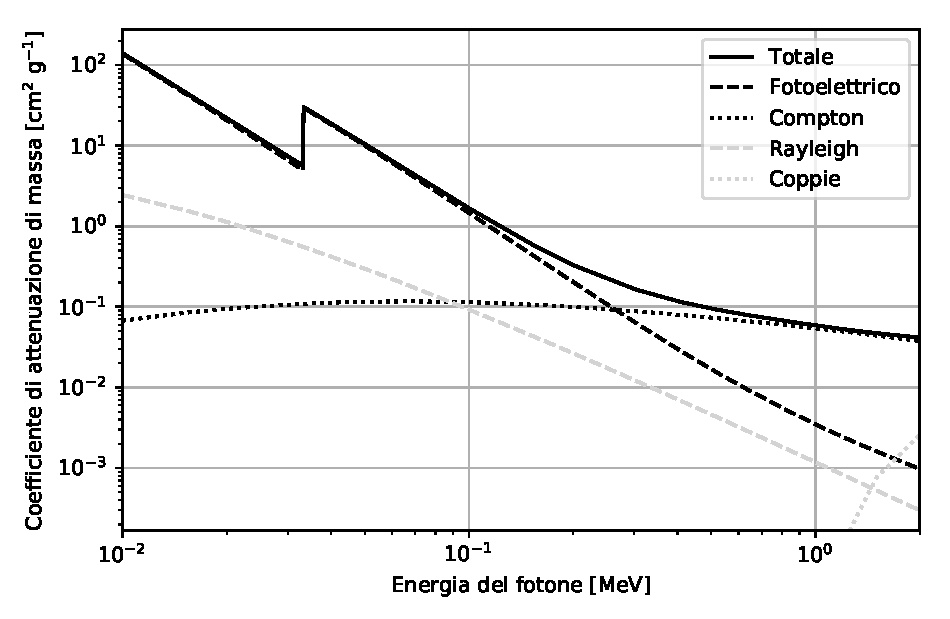
\includegraphics[width=25 em]{immagini/cross}
\caption{\label{fig:cross}
Sezioni d'urto in funzione dell'energia all'interno del nostro cristallo di NaI ($\rho=\SI{3.67}{g\,cm^{-3}})$ espressa come $\sigma=\frac{1}{\rho\lambda}$, dove $\lambda$ è il cammino libero medio all'interno del materiale. Queste informazioni sono tratte da \cite{cross}.}
\label{sezioni}
\end{figure}


\section{Apparato}

\subsection{Apparato A}

% Doveva farlo Bob.

\subsubsection{Descrizione del circuito}

Il circuito del primo apparato costruito è rappresentato in \autoref{circuitone}.

\begin{figure}[h]
\centering
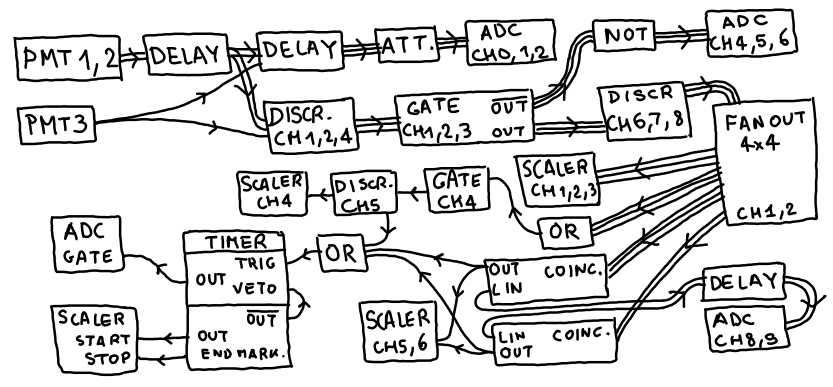
\includegraphics[width=30 em]{immagini/circuitone}
\caption{Schema circuitale dell'apparato A.}
\label{circuitone}
\end{figure}

Le uscite dei PMT sono inviate ai discriminatori, le cui uscite attraversano un modulo di antiretrigger (tempo morto di \SI{1}{\micro s}) e vengono usate per costruire funzioni logiche. I segnali dei PMT vengono anche inviati all'ADC attraverso un attenuatore per evitare di danneggiare lo strumento.
Per quanto riguarda la parte logica, costruiamo e mettiamo in tempo tre tipi di trigger:
\begin{enumerate}
\item canale
\item coincidenza a 2
\item coincidenza a 3.
\end{enumerate}
Il trigger di canale è semplicemente il segnale discriminato del PMT corrispondente; quello di coincidenze è dato dall'uscita di lunga durata del modulo stesso. Mandiamo questi segnali all'ADC in modo che il trigger di canale arrivi in contemporanea con il segnale analogico del canale stesso. Se in quel momento c'è anche un trigger di coincidenza, sappiamo se l'evento ci è arrivato da una coincidenza anziché da un canale singolo. Abbiamo fatto tutto questo per acquisire tutti i canali contemporaneamente ed agevolare la lettura dei dati via software. Purtroppo il \emph{cross-talk}%
\footnote{Spiegheremo come ci siamo accorti di questo problema nella \autoref{ref}.} presente nell'ADC ha rovinato le misure fatte con questo apparato.
Per dare precedenza agli eventi più rari abbiamo collegato questi trigger ad un modulo \emph{or} ritardando i trigger singoli rispetto a quelli di coincidenze a 2 e questi ultimi rispetto alle coincidenze a 3. L'uscita dell'\emph{or} era poi inviata ad un \emph{timer} che generava il gate dell'ADC. L'altro canale di questo \emph{timer} veniva usato per avviare o fermare le acquisizioni.

\subsubsection{Problemi riscontrati}

I problemi descritti in seguito ci hanno spinti a semplificare il circuito per cercare di risolverli.

Il più evidente fin da subito è stato il \emph{bit stuck}: il terzo bit dei dati in formato binario è sempre 1. Gli istogrammi presentano delle lacune di \SI{4}{digit} ogni \SI{4}{digit}. Risolviamo questo problema istogrammando con canali più larghi di \SI{8}{digit}.

Poi abbiamo escluso l'\emph{or} dal circuito perché i segnali che ci arrivavano dalle coincidenze mostravano avere un'energia minore. Abbiamo risolto il problema togliendo l'\emph{or} dal circuito.

Il problema più interessante è dato dal fatto che, confrontando gli spettri del \na{}, abbiamo visto che i fotoni emessi dalla sorgente con attività maggiore avevano energia maggiore.
Il grafico in \autoref{distanze} mostra l'energia dei fotopicchi del sodio in funzione della distanza della sorgente ad attività elevata dal rivelatore usato per fare la misura.
\marginpar{Sto supponendo che prima di questo punto abbiamo scritto che ci sono due sorgenti di sodio.}

\subsection{Circuito B}

Dopo aver eseguito in maniera preliminare le misure richieste, abbiamo deciso di semplificare il circuito per tenere sotto controllo le criticità descritte nella sezione precedente.

\subsubsection{Descrizione del circuito}

Il nuovo circuito segue lo schema in \autoref{circuitone}.
I segnali dei PMT vengono inviati ai discriminatori per ottenere i segnali logici e agli attenuatori per essere poi inviati all'ADC. I segnali logici attraversano un modulo di antiretrigger per poi essere usati come trigger di acquisizioni singole o per effettuare coincidenze. Una copia dei segnali finisce al contatore. Abbiamo usato il timer per far partire/fermare le acquisizioni come abbiamo fatto per il circuito precedente.

\subsubsection{Problemi riscontrati}
\label{ref}
Dopo aver acceso l'apparato il bit stuck è scomparso e l'aumento di risoluzione ci ha permesso di notare un problema che era già presente nel circuito precedente. Abbiamo iniziato a vedere uno sdoppiamento dello spettro, come evidenziato dalla \autoref{doppio}. 

\begin{figure}[h]
\centering
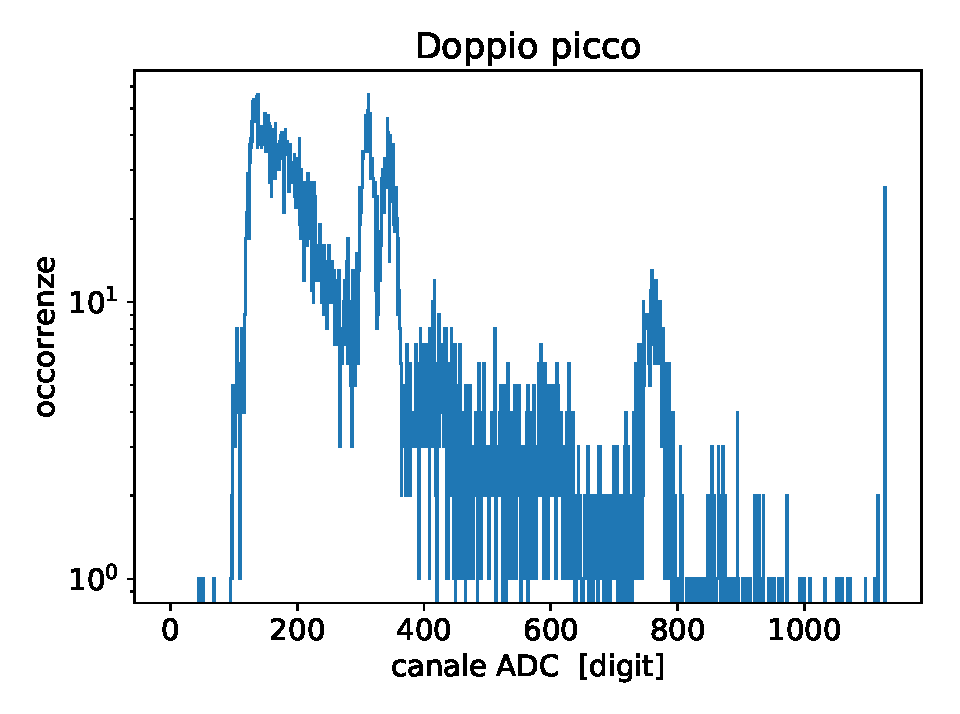
\includegraphics[width=20 em]{immagini/doppio}
\caption{Acquisizione in cui l'annichilazione presenta due picchi.}
\label{doppio}
\end{figure}

Tale problema non era visibile ad occhio nudo nelle precedenti acquisizioni, ma un fit eseguito in seguito ha mostrato la presenza di due gaussiane sovrapposte.

\marginpar{Mi pare che sia coincidenza/anticoincidenza (come detto subito dopo) che ci convince del doppio picco, non uno dei fit.
\texttt{Io mi riferivo a quella misura di stabilità in cui non si vedeva che i picchi erano 2}}

Abbiamo poi scoperto la causa del problema, ovvero il crosstalk.
Come mostra il grafico di \autoref{sdoppio} sinistra, il doppio picco è la somma di quello osservato nelle acquisizioni in coincidenza con quello osservato in anticoincidenza. 

\begin{figure}[h]
\centering
\subfloat
{
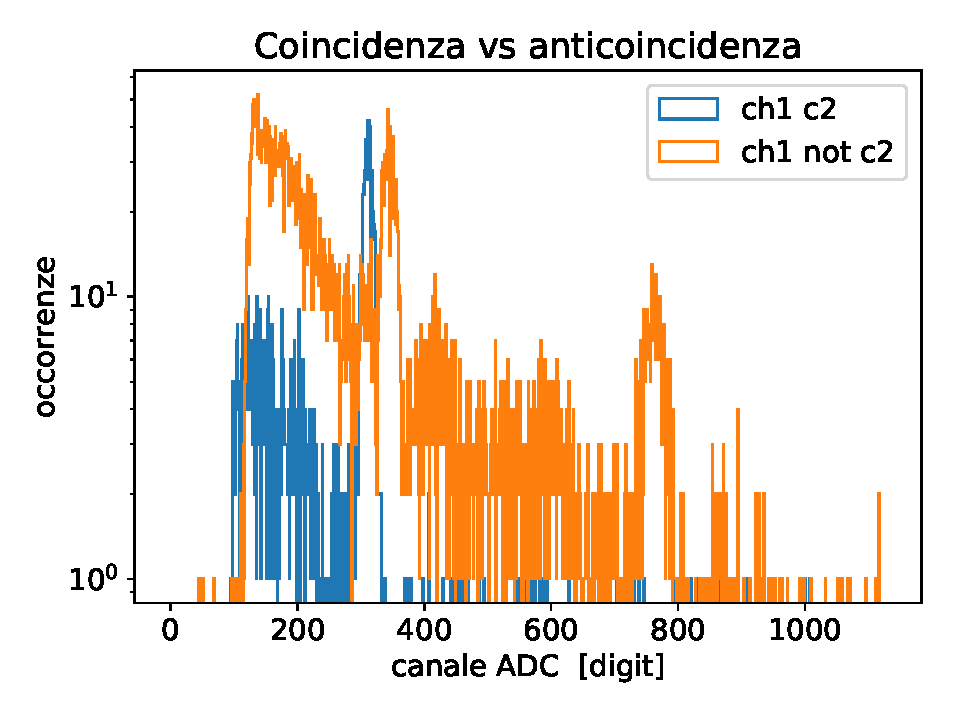
\includegraphics[width=18 em]{immagini/sdoppio}
}
\subfloat
{
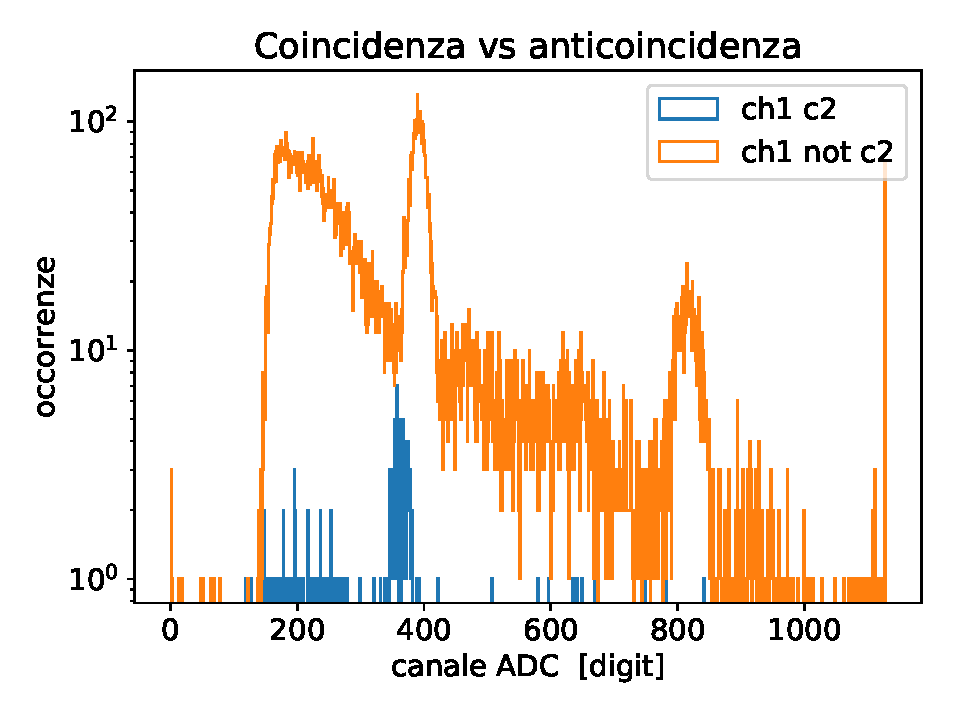
\includegraphics[width=18 em]{immagini/dist}
}
\caption{A sinistra: rappresentazione di dell'acquisizione di \autoref{doppio} separando le coincidenze dalle anticoincidenze. \\
A destra: grafico della stessa misura in cui il PMT1 è vicino alla sorgente mentre il PMT2 è lontano dalla sorgente.}
\label{sdoppio}
\end{figure}

Siamo arrivati alla conclusione che si tratti di un crosstalk dal fatto che il picco in anticoincidenza coincide con quello di un singolo canale quando tutti gli altri sono scollegati.
Inoltre abbiamo visto, aumentando la distanza di un PMT dalla sorgente, che il picco delle coincidenze si rimpicciolisce (perché ha meno eventi) e il picco in anticoincidenza tende ad assomigliare sempre di più a quello dell'acquisizione con canale singolo (\autoref{sdoppio} destra).

\marginpar{Una volta che hai separato lo spettro in coincidenza e anticoincidenza,
mi sembra inutile far vedere che le coincidenze calano se allontani i rivelatori;
sarebbe stato utile se non avessi potuto separare lo spettro.
Metterei insieme il grafico di figura 4 e il primo di figura 5 che sono il confronto interessante.}

In seguito abbiamo provato che questo problema si riscontra anche quando i canali da analizzare non sono collegati ad ingressi adiacenti dell'ADC. Inspiegabilmente, il problema si è ripresentato solo a giorni alterni. 


\section{Misura e analisi}

% Misure preliminari

\subsection{Punto di lavoro}

% Sappiamo dalla precedente esperienza sull'effetto Compton che i PMT con scintillatore di NaI(Tl) lavorano bene in un range di tensioni che va da \SI{600}V a \SI{800}V e l'unica differenza tra una tensione e l'altra è una variazione della scala.
% la frase non ha senso perché la tensione c'entra con il PMT e non con lo scintillatore.
Per i PMT scegliamo delle tensioni che seguano le caratteristiche dichiarate dal tecnico di laboratorio facendo in modo che, in presenza della sorgente, si abbiano dei rate simili tra i 3 PMT.
Allora mettiamo il PMT1 a \SI{703}V, il PMT2 a \SI{839}V ed il PMT3 a \SI{930}V.

Impostiamo le soglie dei discriminatori al minimo (circa \SI{-50}{mV}) perché il rumore casuale è
% da dove esce fuori 1 %??
%al massimo l'\SI{1}{\%} degli eventi che misuriamo usando le sorgenti meno attive
trascurabile.
% gac
%L'utilizzo delle coincidenze rende questo rumore molto più raro.

% l'abbiamo già detto nel circuito
%Usiamo degli attenuatori per cambiare la scala delle misure in caso di necessità.


\subsection{Gate dell'ADC}

Variamo la durata del gate dell'ADC e calcoliamo il rapporto $\sigma\!/$\!media per il picco di annichilazione rivelato dal PMT1, modellato come al solito con una gaussiana.
Su alcune misure abbiamo introdotto dei ritardi per migliorare o peggiorare la sincronizzazione con il gate al fine di quantificare quanto la messa in tempo influisca sulla nostra risoluzione. Il risultato di questa misura è in \autoref{fig:gate}, i dati sono in \autoref{tab:gate}.

\begin{figure}[h]
\centering
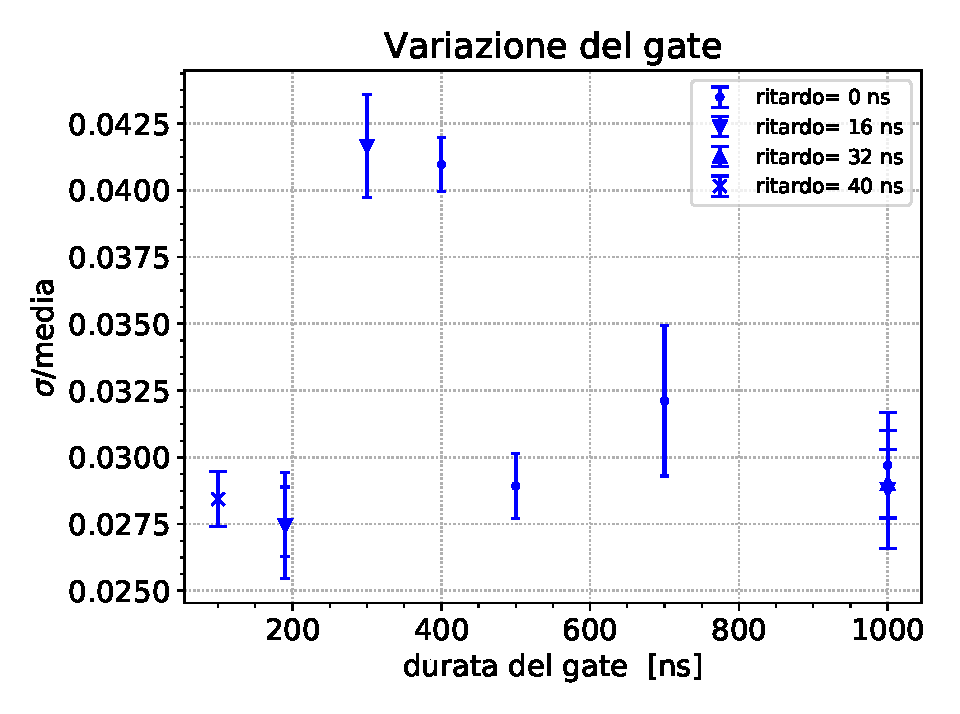
\includegraphics[width=20 em]{immagini/gate}
\caption{Grafico della risoluzione in funzione della durata del gate. Le misure sovrapposte sono state ottenute ritardando il segnale del PMT1.}
\label{fig:gate}
\end{figure}

\begin{table}[h]
\centering
\begin{tabular}{c|c|c|c}
durata (ritardo) [ns] & media [digit] & $\sigma$ [digit] & $\sigma\!/$\!media\\
\hline
 100 & 304.88$\,\pm\,$34 &  8.67$\,\pm\,$31 & 0.0284 $\,\pm\,$10 \\  
 190 & 492.82$\,\pm\,$50 & 13.59$\,\pm\,$65 & 0.0276 $\,\pm\,$13 \\
 190 & 513.05$\,\pm\,$80 & 14.1 $\,\pm\,$1.0 & 0.0274$\,\pm\,$20 \\
 300 & 307.68$\,\pm\,$36 & 12.81$\,\pm\,$59 & 0.0416 $\,\pm\,$19 \\
 400 & 344.25$\,\pm\,$25 & 14.10$\,\pm\,$34 & 0.0410 $\,\pm\,$10 \\
 500 & 524.01$\,\pm\,$42 & 15.16$\,\pm\,$64 & 0.0289 $\,\pm\,$12 \\
 700 & 482.54$\,\pm\,$85 & 15.5 $\,\pm\,$1.4 & 0.0321$\,\pm\,$28 \\
1000 & 539.43$\,\pm\,$61 & 16.0 $\,\pm\,$1.1 & 0.0297$\,\pm\,$20 \\
1000 & 553.88$\,\pm\,$71 & 15.9 $\,\pm\,$1.2 & 0.0288$\,\pm\,$22 \\
1000 & 542.68$\,\pm\,$41 & 15.75$\,\pm\,$69 & 0.0290 $\,\pm\,$13 
\end{tabular}

\caption{Andamento della risoluzione in funzione della durata del gate. I numeri tra parentesi indicano di quanto è stato ritardato il PMT1.}
\label{tab:gate}
\end{table}

Dall'analisi dei dati abbiamo potuto vedere che la risoluzione migliore si raggiunge quando il gate dura meno di \SI{200}{ns}
\marginpar{Con le incertezze riportate, mi sembra che, fatta eccezione per 300 e 400, le misure siano tutte compatibili.}
ma questo valore non è un buon punto di lavoro perché cambiare la durata del gate cambia la scala e, in questo caso, non ci permetteva di vedere il picco del neon.
\marginpar{Il motivo non è il picco del neon, perché accorciare il gate è come attenuare e quindi a maggior ragione si vedono i picchi più a destra. Inoltre usando gli attenuatori si può sempre compensare la variazione del gate.}
L'alternativa migliore sembrerebbe essere una durata del gate di \SI{1}{\micro s}, ma il manuale dell'ADC specifica che a tale valore (o anche maggiore) diminuisce la linearità della digitalizzazione. Per questo abbiamo scelto di usare un gate di \SI{550}{ns} nell'apparato A.
\marginpar{Il manuale dice che aumenta l'errore, non che peggiora la linearità (quella era per segnali sopra \SI1V). Inoltre come limite dà \SI{200}{ns}.}
Questa scelta è poi diventata \SI{1}{\micro s} nell'apparato B per evitare problemi derivanti dal jitter dei segnali. Infine notiamo che cambiare i ritardi sui segnali in ingresso non influisce significativamente sulla risoluzione dell'apparato.
\marginpar{I dati nella tabella non mi tornano. Le sigma sono grosse quanto le medie e infatti i rapporti vengono tutti dell'ordine dell'unità, diversi da quelli riportati nel grafico.}


\subsection{Stabilità}

Mostriamo l'instabilità del nostro sistema di rivelatori nei 2 apparati sopra descritti monitorando la posizione dei fotopicchi del sodio in funzione del tempo.
La prima misura è stata fatta con l'apparato A il 3 maggio e dura \SI{16}{ore}, la seconda  è stata eseguita con l'apparato B il 15 maggio e dura \SI{63}{ore}.
Nella prima misura sono presenti tutti i canali, nella seconda è presente solo il canale 1 per evitare il cross-talk riscontrato nella precedente.
Abbiamo usato l'energia nominale dei 2 picchi per ricavare una ``retta di calibrazione'' di pendenza $m$ e intercetta $q$ e abbiamo osservato l'evoluzione temporale di questi parametri. Usiamo l'espressione tra virgolette perché lo scopo dell'esperienza è fingere di non conoscere la massa dell'elettrone per poi misurarla.

% misura 1
\begin{figure}[h]
\centering
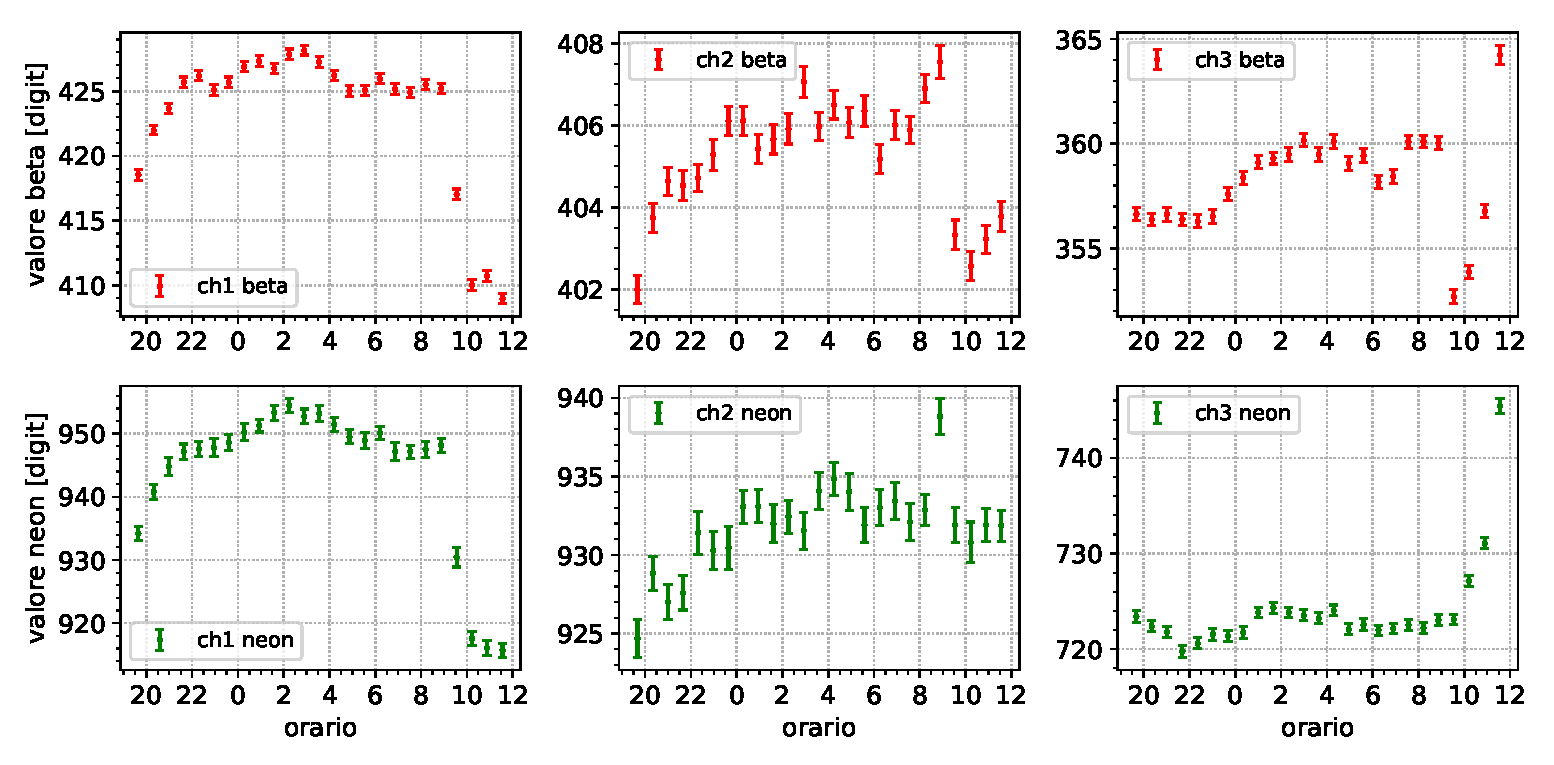
\includegraphics[width=\textwidth]{immagini/0503_picchi}
\caption{Misura di stabilità iniziata il 3 maggio alle 19. I grafici rappresentano la posizione dei picchi in funzione del tempo; ``beta'' indica il picco di annichilazione e ``neon'' indica il fotone emesso dal decadimento del neon.}
\label{picchi1}
\end{figure}

\begin{figure}[h]
\centering
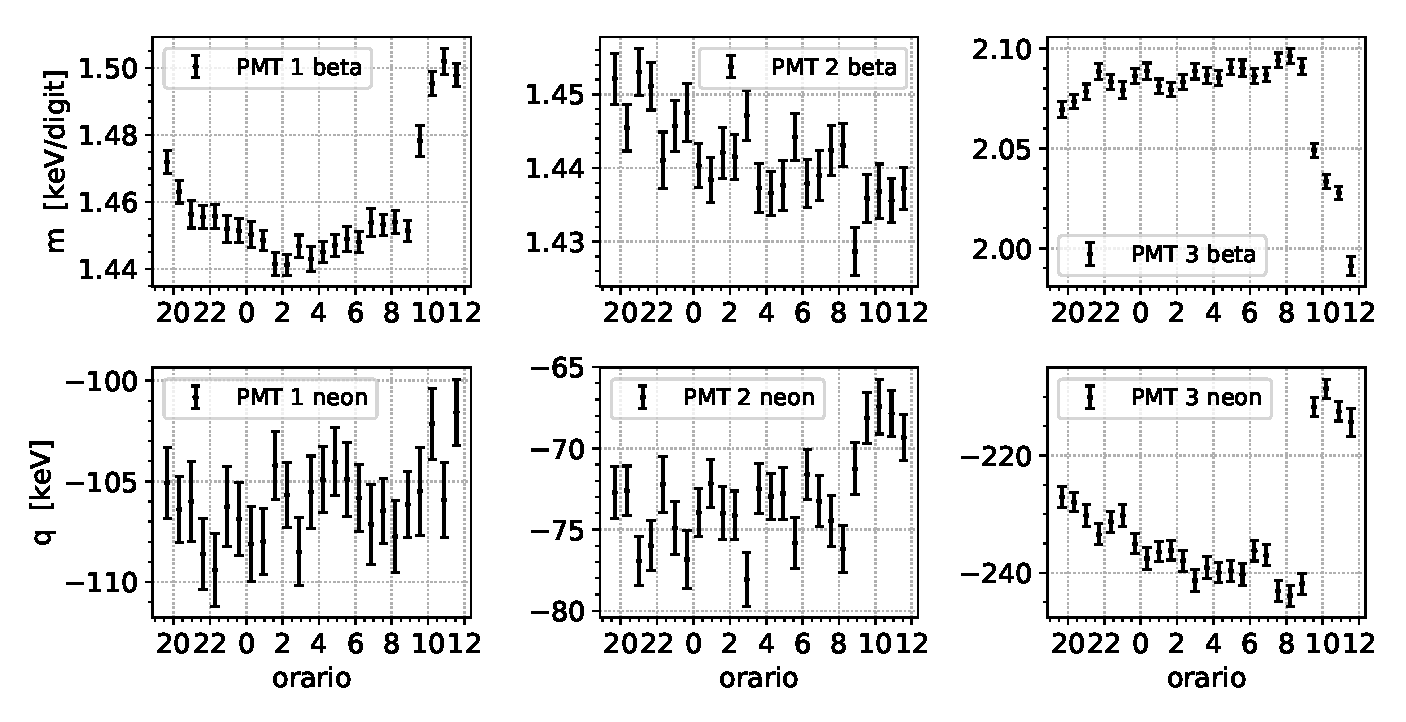
\includegraphics[width=\textwidth]{immagini/0503_rette}
\caption{Misura di stabilità iniziata il 3 maggio alle 19. I grafici rappresentano il valore della pendenza e dell'intercetta della ``retta di calibrazione'' in funzione del tempo.}
\label{rette1}
\end{figure}

% misura 2
\begin{figure}[h]
\centering
\subfloat
{
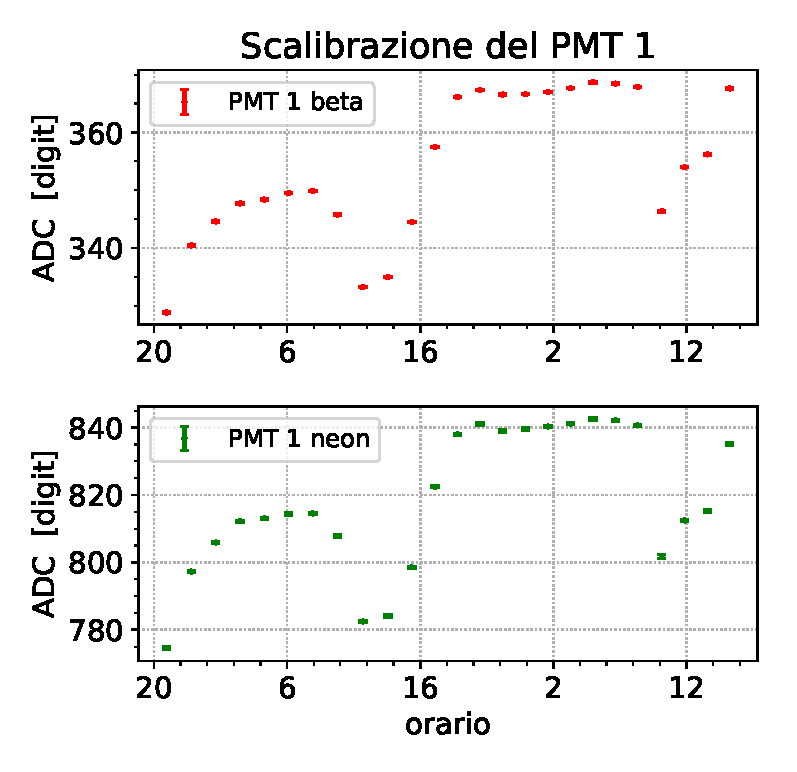
\includegraphics[width=0.49\textwidth]{immagini/0515_picchi}
}
\subfloat
{
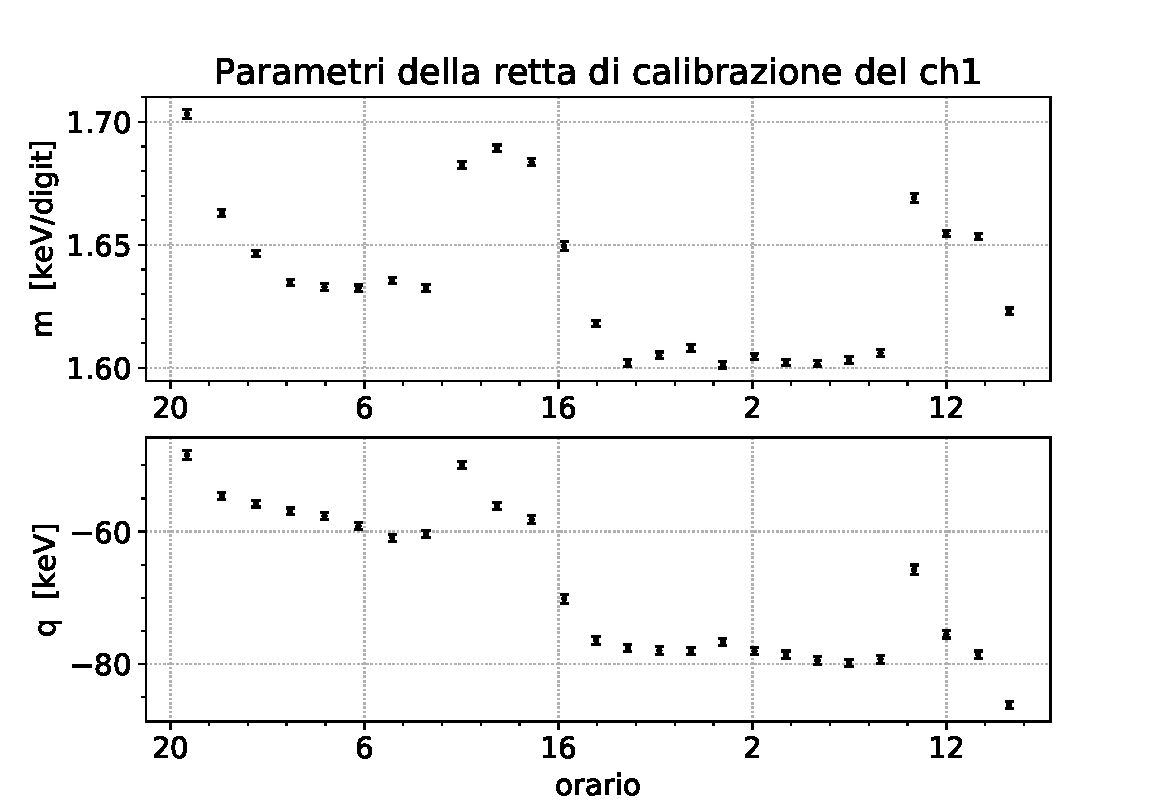
\includegraphics[width=0.49\textwidth]{immagini/0515_rette}
}
\caption{Misura di stabilità iniziata il 15 maggio alle 19.\\
A sinistra:  grafici che rappresentano la posizione dei picchi in funzione del tempo; ``beta'' indica il picco di annichilazione e ``neon'' indica il fotone emesso dal decadimento del neon. \\
A destra: grafici che rappresentano il valore della pendenza e dell'intercetta della ``retta di calibrazione'' in funzione del tempo.}
\label{picchi2}
\end{figure}

% discussione dei dati
Guardando i dati della prima misura (\autoref{picchi1} e \autoref{rette1}) vediamo che i vari rivelatori si scalibrano in modo diverso. L'andamento dei punti indica la notte come momento di massima stabilità e l'apertura del laboratorio come momento di massima instabilità.

Dai dati della seconda misura (\autoref{picchi2} sinistra e \autoref{picchi2} destra) si nota uno spostamento coerente dei fotopicchi del sodio che si stabilizza durante la notte. Anche qui si nota una scalibrazione significativa durante gli orari di apertura del laboratorio.
Le stesse considerazioni valgono anche per i parametri della retta di calibrazione.

\subsection{Rimbalzi}

Guardando lo scatter plot di misure in coincidenza, abbiamo notato dei comportamenti non attesi che abbiamo supposto e poi verificato essere dei fotoni che rimbalzano da un rivelatore all'altro.

La \autoref{scatter} mostra un tipico scatter plot nella configurazione in cui 2 rivelatori sono posti uno di fronte all'altro alla stessa distanza da una sorgente di \na{}.

\begin{figure}[h]
\centering
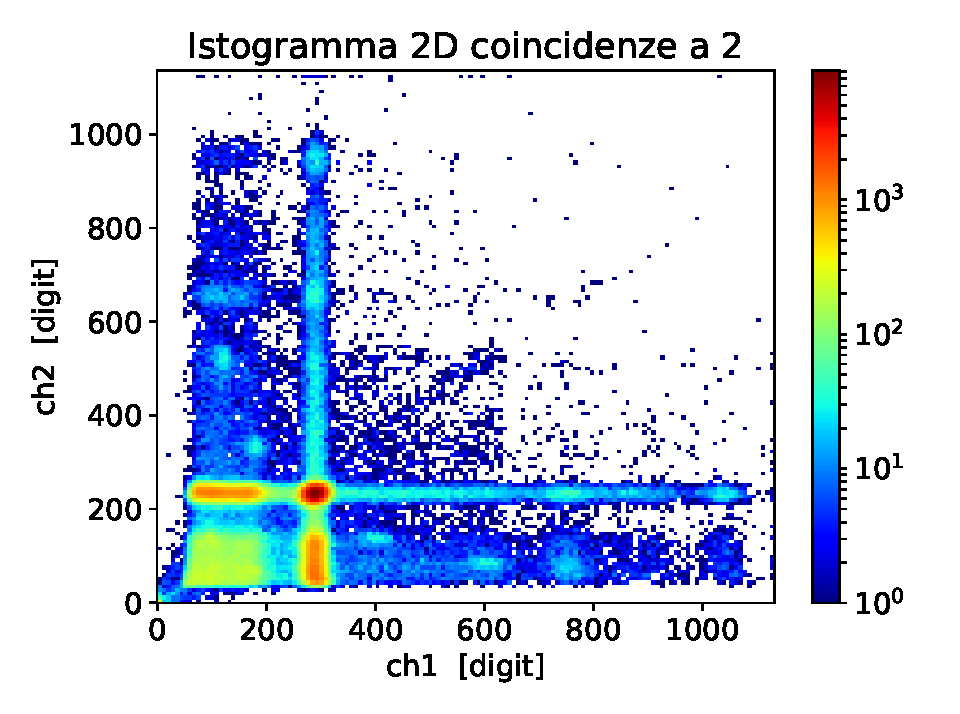
\includegraphics[width=\textwidth]{immagini/esempio}
\caption{Tipico scatter plot di una misura in coincidenza. La descrizione di questo grafico è presente nel testo.}
\label{scatter}
\end{figure}

\marginpar{Chiedere a Jack di fare il super grafico con istogrammi 1D e 2D se non si perde troppo tempo}

Si vedono degli eccessi in alcuni punti del grafico che chiameremo in seguito \emph{strutture}. La più vistosa si manifesta quando entrambi i fotoni di annichilazione effettuano un processo fotoelettrico all'interno degli scintillatori. In basso a sinistra si nota invece la zona in cui entrambi hanno subito una diffusione Compton. Le bande arancioni intorno a questa zona rappresentano invece gli eventi in cui un fotone proveniente dall'annichilazione ha fatto fotoelettrico su un rivelatore e l'altro ha fatto Compton sull'altro.
La stessa cosa avviene con il fotone proveniente dal decadimento del neon, rappresentato dalle strutture nella parte centrale del grafico adiacente ai bordi della figura. La struttura più a destra (o più in alto) rappresenta l'arrivo simultaneo di un fotone di annichilazione insieme ad uno del neon. L'interpretazione degli eventi è analoga a quelli descritti precedentemente.

\marginpar{Non sarebbe male mettere una legenda sui picchi.}

Le strutture non attese sono i due eccessi presenti nella zona in cui il fotone del neon e quello dell'annichilazione fanno entrambi scattering Compton. Queste strutture si manifestano a valori di energia coincidenti ai picchetti della spalla Compton
\marginpar{``Picchetti della spalla Compton'' non è molto chiaro, ma ci penserò più tardi a come aggiustarli.}

Per verificare la nostra ipotesi abbiamo messo i rivelatori nella configurazione di \autoref{spostati}, in modo da poterci aggiungere dei mattoni di piombo come in \autoref{spostati2}. \marginpar{AGGIUSTARE}
Lo scatter plot corrispondente si trova in \autoref{spostato}: la struttura più popolata non è più data dalla rivelazione simultanea dell'annichilazione per effetto fotoelettrico, ma dalla somma degli eventi nelle bande che si incrociano.
In questa configurazione non si nota più uno degli eccessi inattesi nominati prima: quello ad energia più alta. Adesso sono diventate evidenti due strutture circolari nella zona in basso a sinistra del grafico: esse e l'ultimo tipo di struttura rimasta scompaiono completamente quando effettuiamo la misura nella configurazione mostrata in \autoref{spostati2}, come mostrato in \autoref{piombo}.

\begin{figure}[h]
\centering
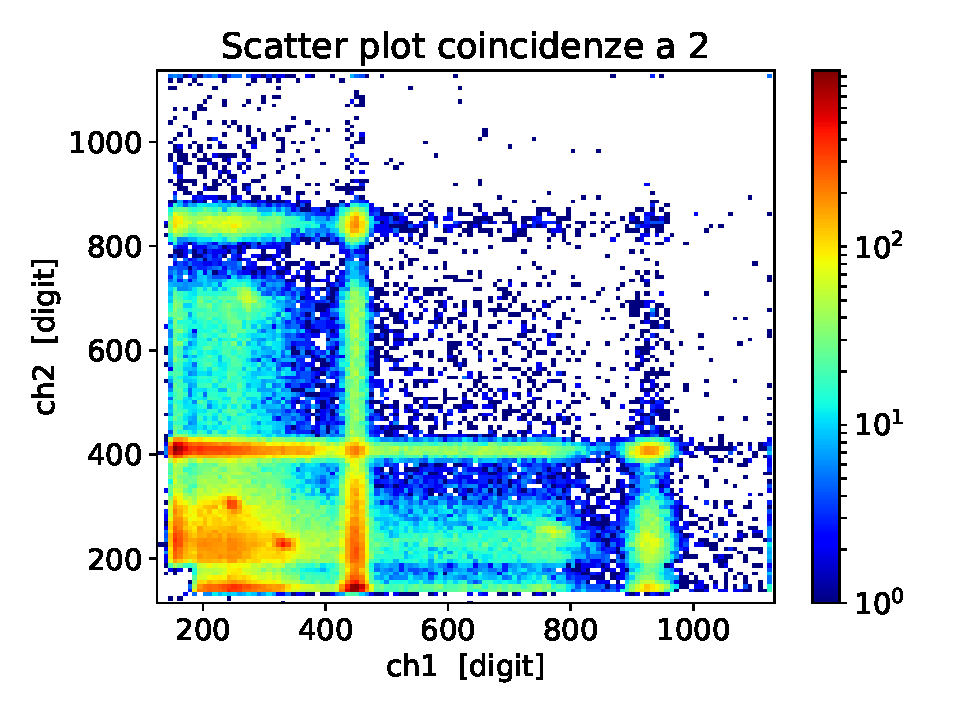
\includegraphics[width=\textwidth]{immagini/0518_rimbalzi}
\caption{Misura eseguita nella configurazione di \autoref{spostati}. La descrizione del grafico è presente nel testo.}
\label{spostato}
\end{figure}

\begin{figure}[h]
\centering
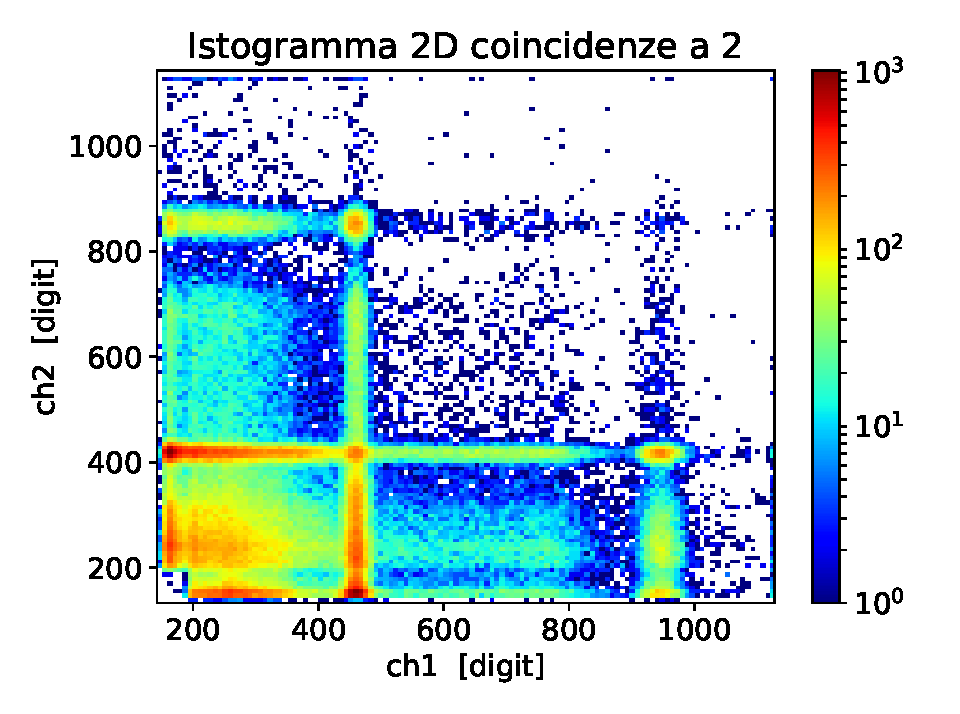
\includegraphics[width=\textwidth]{immagini/0518_piombo}
\caption{Misura eseguita nella configurazione di \autoref{spostati2}. La descrizione di questo grafico è presente nel testo.}
\label{piombo}
\end{figure}


\subsubsection{Misura con un solo fotone}

Abbiamo effettuato la misura nella configurazione di \autoref{solo} e poi \autoref{solo_pb} usando la sorgente di \cs{}: lo scopo della misura è quantificare l'importanza di un rimbalzo tra scintillatori vicini.

 


\subsection{Misure con TDC}

Collegando le uscite discriminate dei PMT 1 e 2 ai due ingressi dell'unico TDC funzionante che abbiamo trovato in laboratorio, possiamo misurare i ritardi tra le risposte di due PMT posti uno di fronte all'altro sfruttando i fotoni dell'annichilazione. Per eseguire la misura usiamo come trigger le coincidenze e ritardiamo i segnali dei due PMT, dato che il trigger è successivo alla rivelazione dei fotoni. \`E stato scelto un ritardo di \SI{60}{ns} in modo che la differenza tra i tempi di arrivo $\Delta t=t_1-t_2$ possa essere sia positiva che negativa.

Prima di eseguire la misura calibriamo il TDC con il generatore di funzioni usando come trigger un'onda quadra e come \emph{stop} lo stesso segnale ma ritardato in modo arbitrario.
Eseguiamo questa calibrazione per le due scale disponibili: \SI{102}{ns} e \SI{510}{ns}.
Le calibrazioni hanno mostrato una buona linearità, ma la misura dei ritardi ha mostrato che il TDC, per un motivo a noi ignoto, non funziona.
Il grafico di Figura\autoref{100} è uguale a quello di Figura\autoref{500} nonostante le acquisizioni siano state fatte con due scale diverse. Se nei due grafici ci fosse la stessa cosa, vedremmo la figura allargata di un fattore dato dal rapporto dei due fondoscala. Inoltre l'offset delle scale del TDC vale circa \SI{1}{digit}, quindi lo spostamento di circa \SI{50}{digit} del picco presente nei grafici non può essere spiegato da nessun effetto fisico.

\begin{figure}[h]
\centering
\subfloat
{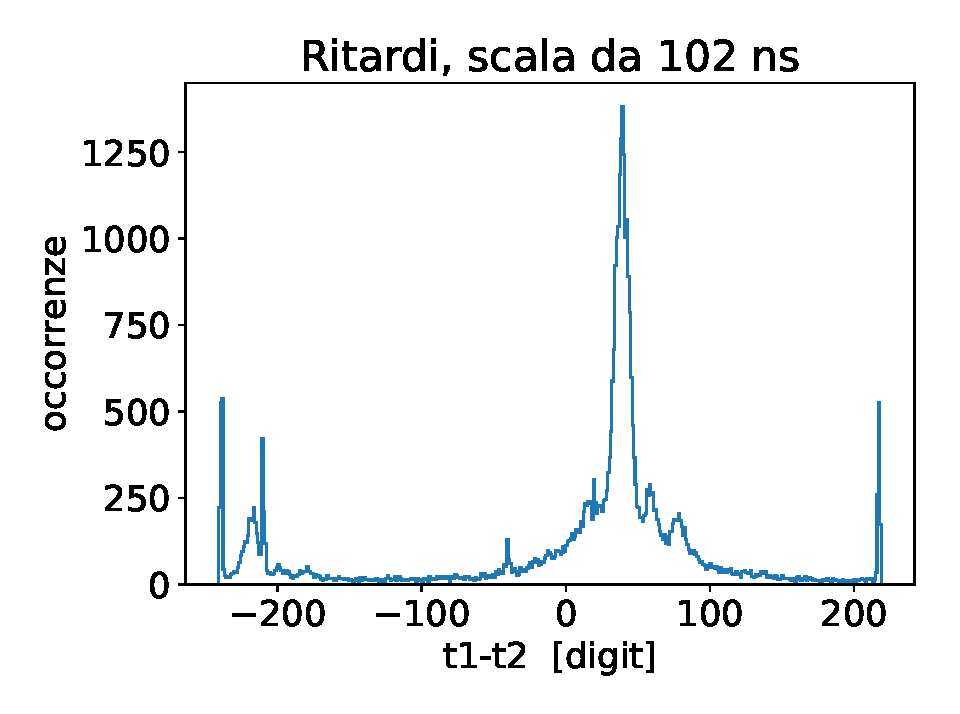
\includegraphics[width=17 em]{immagini/100}
\label{100}} \quad
\subfloat
{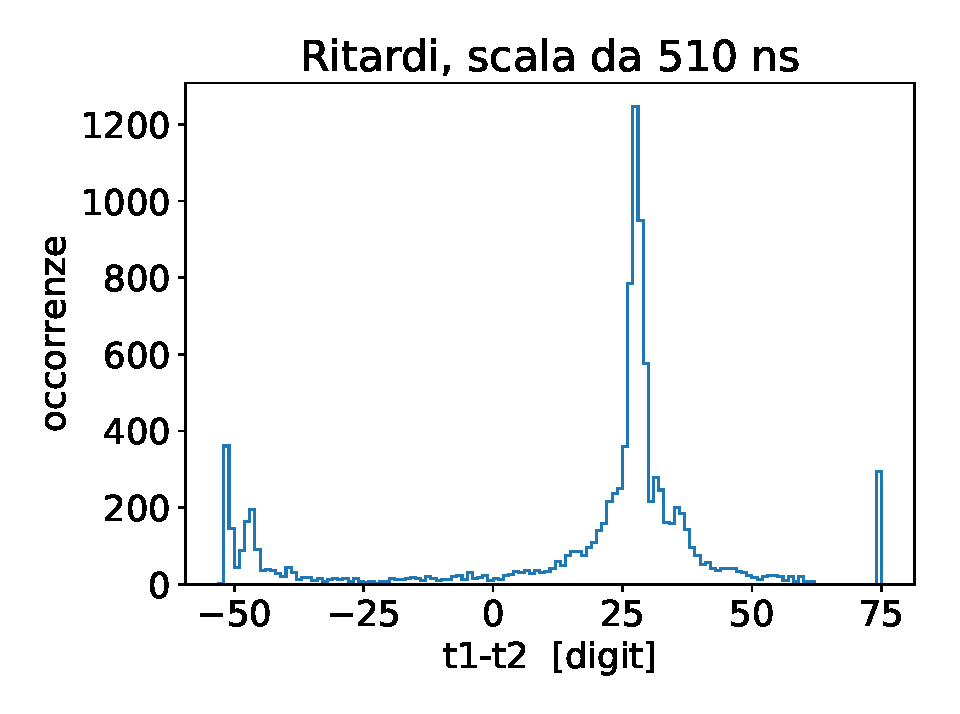
\includegraphics[width=17 em]{immagini/500}
\label{500}}

\caption{Misura di ritardo vista da entrambe le scale del TDC.}
\label{confronto}
\end{figure}

Questo problema ci impedisce di fare i facoltativi.

% Misure importanti

\subsection{Massa dell'elettrone}

Per ricavare la massa dell'elettrone misuriamo l'energia del picco di annichilazione del \na{}
calibrando la scala di energia con i fotopicchi di \co{} e \cs{}.
Poiché la scala di energia varia significativamente nell'arco di tempo in cui facciamo le misure,
misuriamo contemporaneamente lo spettro di tutte le sorgenti.
Triggeriamo su un singolo PMT,
collegando solo quel PMT all'ADC, per evitare il crosstalk tra i canali dell'ADC.
Ripetiamo la misura con i 3 scintillatori disponibili.

\subsubsection{Fit dei picchi}

\begin{figure}
	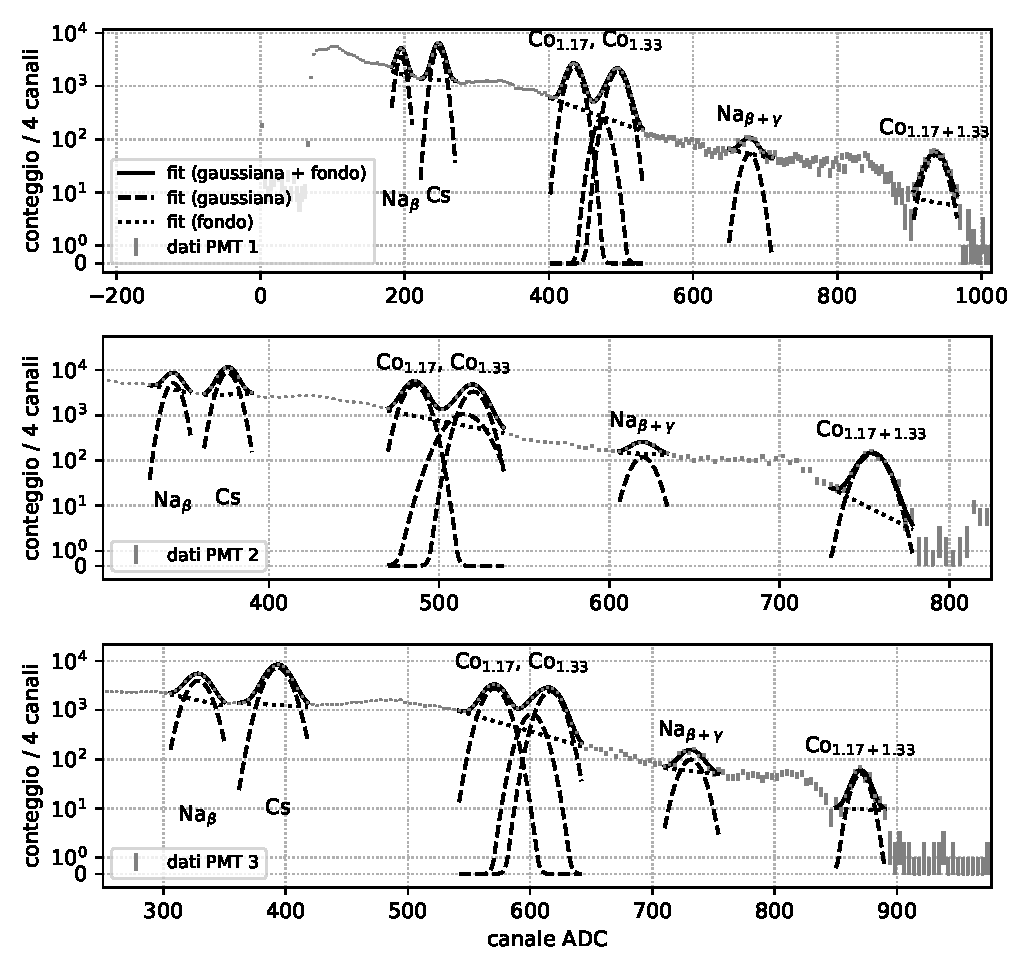
\includegraphics[width=\textwidth]{immagini/mass18-peaks}
	\caption{\label{fig:mass18-peaks}
	Ciao}
\end{figure}

Fittiamo ogni picco, scegliendo a mano l'intervallo di canali su cui fittare,
con una gaussiana più un esponenziale come fondo.
Il fit è ai minimi quadrati sull'istogramma.
I bin fittati contengono tutti almeno 5 eventi.
Controlliamo che cambiare il ribinnaggio dei canali dell'ADC non cambia significativamente il risultato.
I~fit sono riportati in \autoref{fig:mass18-peaks}.
Tutti i fit hanno un pvalue ragionevole;
il test di Kolmogorov-Smirnov sull'uniformità dei pvalue dà un pvalue \SI{18}\%.
Per i picchi del cobalto e quello del neon, che sono sovrapposti, il fit è unico.
Con dei test vediamo che il risultato per la media del picco del neon,
che è praticamente nascosto da quelli del cobalto,
è instabile, quindi lo teniamo nel fit come fondo ma non lo usiamo per ricavare la massa.

\subsubsection{Fit della massa}

\begin{figure}
	\centering
	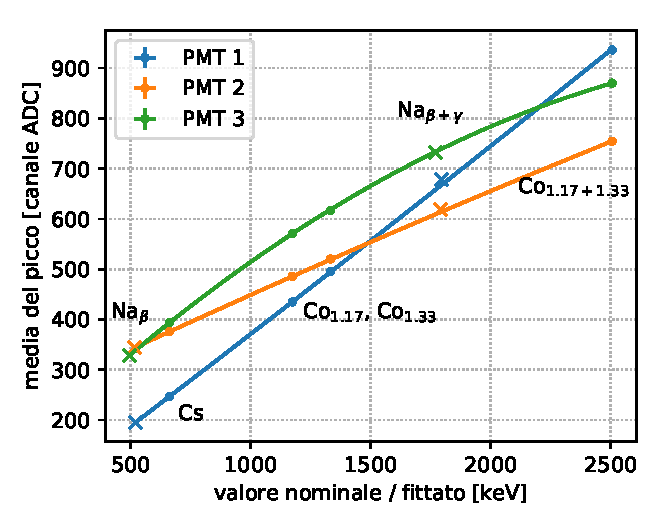
\includegraphics[width=25em]{immagini/mass18-cal}
	\caption{\label{fig:mass18-cal}
	Ciao}
\end{figure}

\begin{table}
	\hspace{-3em}
	\begin{tabular}{c|cccc|cc}
		PMT & $a$ & $b$ [\si{keV^{-1}}] & $c$ [\si{keV^{-2}}] & $m$ [\si{keV}] & $\chi^2$/dof & $F$ \\
		\hline
		1 &   \num{7.31(54)} &  \num{0.3584(11)} &   \num{2.60(26)} & \num{519.95(50)} & 33.3 & 6.9 \\
		2 & \num{228.02(31)} & \num{0.22802(56)} &  \num{-3.55(11)} & \num{516.44(55)} & 24.4 & 6.2 \\
		3 & \num{113.47(44)} & \num{0.46701(84)} & \num{-32.94(18)} & \num{495.25(44)} &  4.1 & 2.3
	\end{tabular}
	\caption{\label{tab:massfit}
	Risultati dei fit di calibrazione e massa dell'elettrone per ogni PMT.
	La curva di calibrazione è $E_\text{adc}=2cE^2+bE+a$.
	In tutti i fit le correlazioni risultano circa \SI{50}\% tra $m$ e gli altri parametri
	e circa \SI{95}\% tra $a$, $b$ e $c$.
	$F$ è il fattore per cui riscalare l'incertezza su $m$
	ricavato testando il fit sui picchi di calibrazione.}
\end{table}

Inizialmente fittiamo le medie dei picchi in funzione dell'energia con una retta
\begin{equation}
	\label{eq:retta}
	E_\text{adc} = b \cdot E + a,
\end{equation}
dove, a seconda dei casi, $E$ è
\begin{itemize}
	\item il valore noto dell'energia per i picchi di calibrazione;
	\item la massa $m$ dell'elettrone (parametro di fit) per il picco di annichilazione;
	\item $m$ più l'energia del fotone del neon per il picco $\na_{\beta+\gamma}$.
\end{itemize}
Nel fit teniamo conto della correlazione tra i picchi del cobalto.
Il pvalue del fit è praticamente 0,
ovvero le incertezze statistiche sono sufficientemente piccole da rigettare il modello \eqref{eq:retta}.

Poiché abbiamo ancora 3 gradi di libertà,
rendiamo il modello più generico aggiungendo il termine quadratico:
\begin{equation}
	\label{eq:parabola}
	E_\text{adc} = 2c \cdot E^2 + b \cdot E + a.
\end{equation}
Anche questo modello viene rigettato con forza per i PMT 1 e 2, ma non per il 3.
Non vogliamo avere meno di due gradi di libertà nel fit,
quindi in mancanza di un modello adeguato stimiamo un'incertezza sistematica aggiuntiva in questo modo:
per ogni picco di calibrazione ripetiamo il fit lasciando libera,
oltre all'energia del picco di annichilazione,
anche l'energia del picco di calibrazione.
Per ognuno di questi fit calcoliamo il rapporto tra
la differenza tra l'energia fittata e l'energia nota del picco di calibrazione
e la deviazione standard stimata dal fit sull'energia fittata.
Riscaliamo l'incertezza sulla massa del fit principale
per la media quadratica di questi rapporti.
Il grafico del fit è riportato in \autoref{fig:mass18-cal},
i risultati dettagliati sono riportati in \autoref{tab:massfit}.
Le masse fittate, con l'incertezza riscalata, risultano
\begin{center}
	\begin{tabular}{cc}
		PMT 1: & $m=\SI{520.0(34)}{keV}$ \\
		PMT 2: & $m=\SI{516.4(34)}{keV}$ \\
		PMT 3: & $m=\SI{495.2(10)}{keV}$
	\end{tabular}
\end{center}

\subsection{Cattura elettronica}

Nel processo di cattura elettronica nel \na{}
viene emesso solo il fotone del neon a \SI{1275}{keV} e non il positrone.
Vogliamo misurare il branching ratio della cattura elettronica.
Le uniche informazioni precise sui rate parziali le possiamo estrarre dai fotopicchi
perché sono le uniche parti dello spettro che distinguiamo chiaramente
e per le quali abbiamo un modello ragionevole (la gaussiana).

\subsubsection{Normalizzazione del rate}

L'ADC riesce a leggere solo una frazione degli eventi,
però è ragionevole supporre che la decimazione sia imparziale,
quindi per ottenere il rate parziale di una regione dello spettro
basta moltiplicare il numero di eventi in quella regione
per il rate misurato dal contatore
e dividere per il numero totale di eventi registrati dall'ADC.

\subsubsection{Fotopicchi}

\begin{figure}
	\centering
	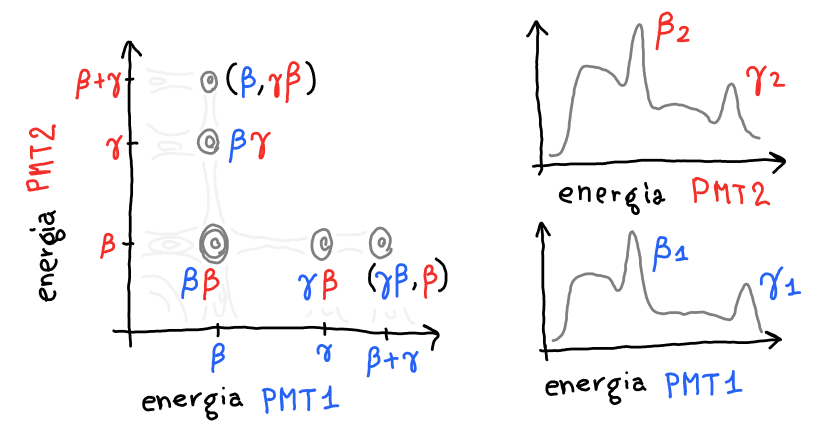
\includegraphics[width=27em]{immagini/schemapicchi}
	\caption{\label{fig:schemapicchi}
	Schema dei fotopicchi usati per misurare il branching ratio di cattura elettronica della sorgente \na{}.
	$\beta$ sono i fotoni emessi dall'annichilazione dei positroni
	e $\gamma$ quelli emessi dal neon eccitato in cui decade il \na.}
\end{figure}

Usando due scintillatori\footnote{Non abbiamo considerato configurazioni con tre rivelatori per questa misura.} possiamo ricavare il rate di undici fotopicchi diversi,
corrispodenti alle varie configurazioni con cui i fotoni possono interagire con i rivelatori;
di questi undici ne useremo però al più nove,
riportati schematicamente in \autoref{fig:schemapicchi}.
Indichiamo con $\beta$ i fotoni di annichilazione (\SI{511}{keV})
e con $\gamma$ i fotoni del neon (\SI{1275}{keV}).
Chiamiamo i rivelatori ``1'' e ``2''.
Cinque fotopicchi si ottengono dalle coincidenze a due:
\begin{description}
	\item[$\beta\beta$:]
	Caso in cui entrambi i rivelatori vedono i fotoni di annichilazione contrapposti e li assorbono.
	Questo picco è presente solo se la sorgente è tra i due rivelatori.
	\item[$\gamma\beta$:]
	Caso in cui il rivelatore 1 assorbe il fotone $\gamma$ e il 2 uno dei $\beta$.
	\item[$\beta\gamma$:]
	Come $\gamma\beta$ ma con $\beta$ sul rivelatore 1 e $\gamma$ sul 2.
	\item[$(\beta,\gamma\beta)$:]
	Il rivelatore 1 assorbe $\beta$ e il rivelatore 2 assorbe l'altro $\beta$ e $\gamma$.
	Come $\beta\beta$, questo segnale è presente solo se la sorgente si trova interposta tra i rivelatori.
	\item[$(\gamma\beta,\beta)$:]
	Come il precedente ma con i rivelatori scambiati di ruolo.
\end{description}
Gli altri quattro fotopicchi si ottengono triggerando su uno scintillatore alla volta:
per ogni scintillatore di ottiene un picco $\beta$ e un $\gamma$,
distinguiamo i rivelatori con un pedice: $\beta_1$, $\gamma_1$, $\beta_2$, $\gamma_2$.

\subsubsection{Equazioni dei rate}
\label{sec:eqrate}

Per ogni fotopicco misuriamo il rate.
Scrivendo i rate in funzione delle efficienze e accettanze dei rivelatori
e in funzione del rate di $\beta$ e del rate di $\gamma$
(diversi perché c'è la cattura elettronica)
otteniamo un sistema di equazioni da cui dobbiamo ricavare i rate.
Poiché in generale l'accettanza e l'efficienza non sono fattorizzate, le teniamo combinate.
Usiamo le variabili:
\newcommand*\tot{^\text{tot}}
\newcommand*\R{r}
\newcommand*\Rtot{\mathcal{R}}
\begin{description}
	\item[$\R$:]
	Rate $\beta$.
	\item[$\Rtot$:]
	Rate $\gamma$, ovvero $r$ più il rate di cattura elettronica.
	\item[$p_{\beta1}$, $p_{\beta2}$, $p_{\gamma1}$, $p_{\gamma2}$:]
	Probabilità di assorbimento per i vari fotoni/rivelatori.
	\item[$p_{\beta12}$:]
	Probabilità di assorbimento in coincidenza dei due fotoni $\beta$.
	\item[$p_{\beta1}^\text{tot}$, $p_{\beta2}^\text{tot}$, $p_{\gamma1}^\text{tot}$, $p_{\gamma2}^\text{tot}$:]
	Probabilità di rivelazione totali per i vari fotoni/rivelatori,
	cioè in pratica, rispetto alle variabili senza apice, è incluso il caso in cui il fotone fa Compton.
	\item[$p_{\beta12}^\text{tot}$:]
	Probabilità di rivelazione totale per i fotoni in coincidenza
	\emph{con l'esclusione del caso in cui fanno entrambi Compton}.
	\item[$R_{\beta1}$, $R_{\beta2}$, $R_{\gamma1}$, $R_{\gamma2}$, $R_{\beta\beta}$, $R_{\gamma\beta}$, $R_{\beta\gamma}$, $R_{\beta,\gamma\beta}$, $R_{\gamma\beta,\beta}$:]
	Rate dei vari fotopicchi.
\end{description}
Le equazioni sono
\begin{align}
	R_{\beta\beta} \label{eq:betabeta}
	&= \R p_{\beta12} (1 - p_{\gamma1}\tot - p_{\gamma2}\tot) \\
	R_{\gamma\beta} \label{eq:gammabeta}
	&= 2\R p_{\beta2} p_{\gamma1} - \R p_{\beta12}\tot p_{\gamma1} \\
	R_{\beta\gamma} \label{eq:betagamma}
	&= 2\R p_{\beta1} p_{\gamma2} - \R p_{\beta12}\tot p_{\gamma2} \\
	R_{\beta,\gamma\beta} \label{eq:betagammabeta}
	&= \R p_{\beta12} p_{\gamma2} \\
	R_{\gamma\beta,\beta} \label{eq:gammabetabeta}
	&= \R p_{\beta12} p_{\gamma1} \\
	R_{\beta1}
	&= 2\R p_{\beta1} (1 - p_{\gamma1}\tot) \\
	R_{\gamma1} \label{eq:gamma1}
	&= p_{\gamma1}(\Rtot - 2 \R p_{\beta1}\tot) \\
	R_{\beta1}
	&= 2\R p_{\beta2} (1 - p_{\gamma2}\tot) \\
	R_{\gamma2} \label{eq:gamma2}
	&= p_{\gamma2} (\Rtot  - 2 \R p_{\beta2}\tot).
\end{align}
Nel caso in cui la sorgente non sia interposta tra i rivelatori
bisogna eliminare le equazioni \eqref{eq:betabeta}, \eqref{eq:betagammabeta}, \eqref{eq:gammabetabeta}
e porre $p_{\beta12}\tot = 0$ in \eqref{eq:gammabeta} e \eqref{eq:betagamma}.

Notiamo che $\Rtot$ compare solo nelle equazioni \eqref{eq:gamma1} e \eqref{eq:gamma2}.
Notiamo anche che $\R$ compare solo a moltiplicare le variabili
$p_{\beta1}$, $p_{\beta2}$, $p_{\beta12}$, $p_{\beta1}\tot$, $p_{\beta2}\tot$, $p_{\beta12}\tot$
e che, viceversa, queste compaiono solo a moltiplicare $\R$,
cioè questo insieme di 7 variabili è degenere e va ridotto alle 6 variabili
$\R p_{\beta1}$, $\R p_{\beta2}$, $\R p_{\beta12}$, $\R p_{\beta1}\tot$, $\R p_{\beta2}\tot$, $\R p_{\beta12}\tot$,
quindi non si può ricavare $\R$.
Il sistema è a 9 equazioni con 11 incognite,
quindi bisogna necessariamente fare approssimazioni o aggiungere equazioni anche per ricavare $\Rtot$.

\subsubsection{Informazioni esterne}
\label{sec:ptotp}

Per aggiungere equazioni e ricavare $\Rtot$
prendiamo valori tabulati di $p_{\dots} / p_{\dots}\tot$ da \cite{3}.
\cite{3} fornisce il rapporto per scintillatori da $\SI{2}{''}\times\SI2{''}$ a \SI{10}{cm},
quindi quando usiamo distanze diverse aggiungiamo un'incertezza stimata grossolanamente ai rapporti tabulati.
I rapporti sono
$p_\beta / p_\beta\tot = \SI{50(2)}\%$ e
$p_\gamma / p_\gamma\tot = \SI{22(2)}\%$.
Ricaviamo $p_{\beta12} / p_{\beta12}\tot$ facendo l'approssimazione che valga
$p_{\beta12}\propto p_{\beta1}p_{\beta2}$ cioè che le probabilità si fattorizzino.
Allora
\marginpar{Non si capisce una fava.}
\begin{align*}
	\frac{p_{\beta12}\tot}{p_{\beta12}}
	&= \frac
	{p_{\beta1}p_{\beta2} + (p_{\beta1}\tot - p_{\beta1}) p_{\beta2} + p_{\beta1} (p_{\beta2}\tot - p_{\beta2})}
	{p_{\beta1}p_{\beta2}} = \\
	&= \frac{p_{\beta1}\tot}{p_{\beta1}} + \frac{p_{\beta2}\tot}{p_{\beta2}} - 1.
\end{align*}

\subsubsection{Fattorizzazione delle probabilità}

I rapporti $p_{\dots} / p_{\dots}\tot$ non sono sufficienti per ricavare $\R$.
Per rompere la degenerazione bisogna scrivere le probabilità in termini di accettanze e efficienze.
Nel modello più semplice le probabilità sono fattorizzate in accettanza$\times$efficienza
e $p_{\beta12}$ è fattorizzato in termini dei due rivelatori.
Chiamiamo $A_1$ e $A_2$ le accettanze dei due rivelatori,
$A_{12}$ l'accettanza per i fotoni di annichilazione in coincidenza,
$P_1$ e $P_2$ le efficienze.
Allora
\begin{align*}
	p_{\beta1}
	&= A_1 P_1, \\
	p_{\beta2}
	&= A_2 P_2, \\
	p_{\beta12}
	&= A_{12} P_1 P_2.
\end{align*}
Se dalle equazioni ricaviamo $\R p_{\beta1}$, $\R p_{\beta2}$ e $\R p_{\beta12}$ abbiamo che
\begin{align}
	\label{eq:R}
	\frac {\R p_{\beta1} \cdot \R p_{\beta2}} {\R p_{\beta12}}
	&= \R \frac{A_1 A_2}{A_{12}},
\end{align}
quindi possiamo ricavare $r$ misurando le accettanze.

\subsubsection{Misura}

\begin{figure}
	\hspace{-0.25\textwidth}
	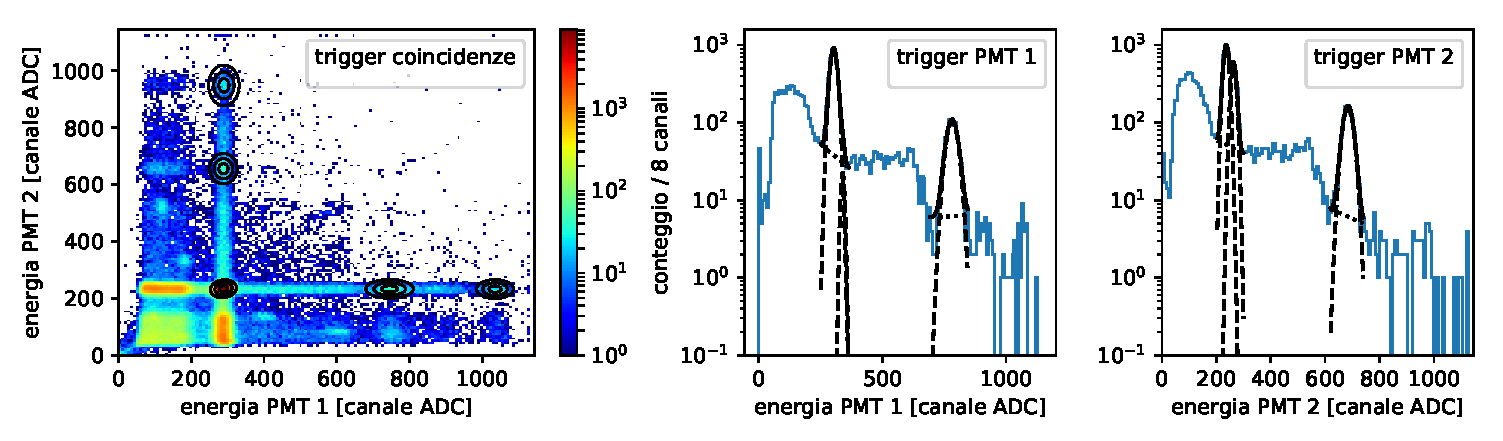
\includegraphics[width=1.5\textwidth]{immagini/ec}
	\caption{\label{fig:ec}
	Dati e fit dei picchi per misurare il braching ratio di cattura elettronica.
	I picchi $\beta_1$ e $\beta_2$ sono fittati con due gaussiane per il crosstalk descritto in \autoref{ref}.
	I risultati dei fit sono in \autoref{tab:fitpicchi2d} e \autoref{tab:fitpicchi1d}.}
\end{figure}

Questa misura è stata fatta con il circuito A.

\paragraph{Apparato}

Poniamo i due scintillatori allineati uno davanti all'altro usando la guida metallica,
con le facce a distanza \SI{9.0 \pm 0.1}{cm}.
La guida permette di farli scorrere, quindi controlliamo che siano allineati
facendo appoggiare le facce e poi allontanandoli.
Attacchiamo un righello da uno scintillatore all'altro per posizionare la sorgente al centro.
Attacchiamo la sorgente a un supporto che possiamo far scorrere fino ad appoggiarlo ai rivelatori
per controllare che sia allineata al centro.
Controlliamo gli allineamenti con foto da varie angolazioni.

\paragraph{Accettanze}

L'accettanza, intesa come probabilità che il fotone attraversi il rivelatore, è ben definita,
però la fattorizzazione della probabilità di rivelazione in accettanza e probabilità di interazione
è approssimativa perché a seconda dell'angolo di incidenza il fotone può attraversare spessori diversi di scintillatore.
Ne teniamo conto calcolando l'accettanza dall'area sottesa dalla circonferenza dello scintillatore
a 1/3 e 2/3 della profondità, prendiamo la media delle due come accettanza e la differenza come incertezza.
Poiché la sorgente è ben allineata, l'accettanza per le coincidenze a 2 è circa il doppio di quelle singole.
Risulta $A_1 = A_2 = A_{12}/2 = \num{0.028(12)}$.

\paragraph{Fit dei picchi}

\newcommand*\gauss{\operatorname{gauss}}
\begin{table}
	\hspace{-2em}
	\begin{tabular}{l|l}
		Picchi & Modello \\
		\hline
		$\gamma_1$, $\gamma_2$
		& $Ae^{-\lambda x} + N\gauss(x, \mu, \sigma)$ \\
		$\beta_1$, $\beta_2$
		& $Ae^{-\lambda x} + N_a\gauss(x, \mu_a, \sigma_a) + N_b\gauss(x, \mu_b, \sigma_b)$ \\
		$\gamma\beta$, $(\gamma\beta,\beta)$
		& $\big(A_1e^{-\lambda_1 x_1} + N\gauss(x_1,\mu_1,\sigma_1)\big)\gauss(x_2,\mu_2,\sigma_2)$ \\
		$\beta\gamma$, $(\beta,\gamma\beta)$
		& $\big(A_2e^{-\lambda_2 x_2} + N\gauss(x_2,\mu_2,\sigma_2)\big)\gauss(x_1,\mu_1,\sigma_1)$ \\
		$\beta\beta$
		& $N\gauss(\mathbf x,\boldsymbol\mu,\boldsymbol\sigma)
		+ A_2e^{-\lambda_2 x_2}\gauss(x_1,\mu_1,\sigma_1)
		+ A_1e^{-\lambda_1 x_1}\gauss(x_2,\mu_2,\sigma_2)$
	\end{tabular}
	\caption[cippalippa]{\label{tab:modelli}
	Modelli usati per fittare i vari picchi.
	Con $\gauss(x,\mu,\sigma)$ si intende una gaussiana di media $\mu$ e deviazione standard $\sigma$.
	Le variabili in grassetto sono bidimensionali.
	$\boldsymbol\sigma$ è la matrice di covarianza
	$\begin{psmallmatrix} \sigma_1 & \sigma_{12} \\ \sigma_{12} & \sigma_2 \end{psmallmatrix}$.
	Per $\beta_1$ e $\beta_2$ ci sono due gaussiane per il crosstalk descritto in \autoref{ref}
	(vedi \autoref{fig:ec}).
	Per $\beta\beta$ la gaussiana del picco ha il parametro di correlazione $\sigma_{12}$ libero
	mentre non ce l'ha negli altri picchi in coincidenza.
	L'abbiamo lasciato libero perché, fittando con correlazione nulla, risulta una significativa discrepanza.}
\end{table}

\begin{table}
	% tabella generata da ec.py
	\hspace{-1.5em}
	\sisetup{separate-uncertainty=false}
	\begin{tabular}{c||ccccc}
		Picco                                 &     $\beta\beta$ &     $\gamma\beta$ & $\gamma\beta,\beta$ &     $\beta\gamma$ & $\beta,\gamma\beta$ \\ \hline\hline
		$N$                                   & \num{7.40(5)e+6} &  \num{3.7(12)e+4} &     \num{3.1(9)e+4} &   \num{3.8(7)e+4} &    \num{5.0(15)e+4} \\ \hline
		$\mu_1$ [$u$]                         &  \num{288.57(5)} &   \num{745.4(28)} &    \num{1035.2(22)} &    \num{288.4(4)} &      \num{289.7(7)} \\
		$\sigma_1$ [$u$]                      &   \num{11.87(6)} &       \num{22(4)} &         \num{17(3)} &     \num{12.7(4)} &       \num{14.0(8)} \\
		$A_1$ [$u$]                           &    \num{123(23)} &       \num{17(4)} &          \num{6(4)} &                 - &                   - \\
		$\lambda_1$ [$u^{-1}$]                &  \num{-0.009(4)} & \num{-0.0034(28)} &      \num{0(10)e-3} &                 - &                   - \\ \hline
		$\mu_2$ [$u$]                         &  \num{233.89(3)} &    \num{233.2(4)} &      \num{232.7(6)} &   \num{655.8(17)} &     \num{948.7(14)} \\
		$\sigma_2$ [$u$]                      &   \num{10.53(3)} &     \num{10.9(4)} &       \num{11.1(7)} &    \num{17.7(24)} &         \num{24(4)} \\
		$A_2$ [$u$]                           &      \num{53(6)} &                 - &                   - &    \num{13.8(22)} &          \num{2(4)} \\
		$\lambda_2$ [$u^{-1}$]                & \num{0.0148(28)} &                 - &                   - & \num{-0.0014(24)} &     \num{0.013(24)} \\ \hline
		$\sigma_{12}/\sqrt{\sigma_1\sigma_2}$ &   \num{0.098(3)} &                 - &                   - &                 - &                   - \\ \hline
		$\chi^2$                              &             87.3 &              54.5 &                40.1 &              74.6 &                44.9 \\
		dof                                   &               61 &                60 &                  32 &                62 &                  52
	\end{tabular}
	\caption{\label{tab:fitpicchi2d}
	Risultati dei fit dei picchi in coincidenza
	per la misura di branching ratio della cattura elettronica.
	$u$ indica le unità dei canali dell'ADC.
	I parametri sono spiegati nella \autoref{tab:modelli}.
	Il rate del picco si ottiene moltiplicando $N$ per il rate totale
	e dividendo per il numero di eventi registrati dall'ADC e per l'area dei bin.}
	\sisetup{separate-uncertainty=true}
\end{table}

\begin{table}
	% tabella generata da ec.py
	\centering
	\sisetup{separate-uncertainty=false}
	\begin{tabular}{c||cccc}
		Picco                      &        $\beta_1$ &      $\gamma_1$ &        $\beta_2$ &      $\gamma_2$ \\ \hline\hline
		$N$, $N_a+N_b$             & \num{3.02(6)e+4} & \num{5.5(3)e+3} & \num{3.60(7)e+4} & \num{7.0(3)e+3} \\ \hline
		$\mu$, $\mu_a$ [$u$]       &   \num{303.1(3)} & \num{781.6(11)} &   \num{236.3(5)} &  \num{684.1(7)} \\
		$\sigma$, $\sigma_a$ [$u$] &  \num{13.51(29)} &  \num{21.2(11)} &     \num{9.8(4)} &   \num{17.5(7)} \\
		$A$ [$u$]                  &      \num{52(5)} &   \num{6.0(22)} &      \num{59(8)} &   \num{7.7(20)} \\
		$\lambda$ [$u^{-1}$]       & \num{0.0060(19)} &   \num{0(4)e-3} & \num{0.0039(20)} &  \num{0.004(5)} \\ \hline
		$\mu_b$ [$u$]              &     \num{339(5)} &               - &   \num{263.6(7)} &               - \\
		$\sigma_b$ [$u$]           &       \num{7(4)} &               - &     \num{9.4(5)} &               - \\ \hline
		$\chi^2$                   &              2.5 &             7.4 &              0.9 &             6.1 \\
		dof                        &                7 &              11 &                5 &              10
	\end{tabular}
	\caption{\label{tab:fitpicchi1d}
	Risultati dei fit dei picchi senza coincidenza
	per la misura di branching ratio della cattura elettronica.
	$u$ indica le unità dei canali dell'ADC.
	I parametri sono spiegati nella \autoref{tab:modelli}.
	Il rate del picco si ottiene moltiplicando $N$ per il rate totale
	e dividendo per il numero di eventi registrati dall'ADC e per la larghezza dei bin.}
	\sisetup{separate-uncertainty=true}
\end{table}

Poiché, come si vede in \autoref{fig:ec},
tutti i picchi hanno un fondo significativo,
ricaviamo il rate dei picchi fittandoli con gaussiane più fondo.
I fit sono ai minimi quadrati sugli istogrammi.
Riportiamo i modelli usati in \autoref{tab:modelli}
e i risultati dei fit in \autoref{tab:fitpicchi2d} e \autoref{tab:fitpicchi1d}.
Per i picchi $\beta_1$ e $\beta_2$ abbiamo fittato con due gaussiane
per il problema descritto in \autoref{ref} dovuto al crosstalk sull'ADC.
I rate ricavati dalle normalizzazioni sono riportati in \autoref{tab:ecfit}.

\paragraph{Fit dei rate e delle probabilità di rivelazione}

\begin{table}
	% tabella generata da ec.py
	\hspace{-2em}
	\begin{tabular}{ccc|cc}
		Dato & Input & Valore fittato & Parametro & Valore fittato \\
		\hline
		             $R_{\beta\beta}$ &     \num{4099(26)} &     \num{4096(26)} &      $\R p_{\beta12}$ &  \num{4.31(5)e+3} \\
		            $R_{\gamma\beta}$ &        \num{20(6)} &        \num{18(3)} &       $\R p_{\beta1}$ & \num{5.69(12)e+3} \\
		      $R_{\gamma\beta,\beta}$ &        \num{17(5)} &        \num{23(4)} &       $\R p_{\beta2}$ & \num{5.77(11)e+3} \\
		            $R_{\beta\gamma}$ &        \num{21(4)} &        \num{19(3)} &         $p_{\gamma1}$ &   \num{0.0052(9)} \\
		      $R_{\beta,\gamma\beta}$ &        \num{28(8)} &        \num{25(5)} &         $p_{\gamma2}$ &  \num{0.0058(11)} \\
		                $R_{\beta_1}$ & \num{1.106(23)e+4} & \num{1.110(22)e+4} &               $\Rtot$ &   \num{4.0(7)e+5} \\
		               $R_{\gamma_1}$ &  \num{2.02(12)e+3} &  \num{1.99(12)e+3} &   $\R p_{\beta1}\tot$ &  \num{8.2(14)e+3} \\
		                $R_{\beta_2}$ & \num{1.122(21)e+4} & \num{1.124(21)e+4} &     $p_{\gamma1}\tot$ &    \num{0.024(6)} \\
		               $R_{\gamma_2}$ &  \num{2.17(10)e+3} &   \num{2.19(9)e+3} &   $\R p_{\beta2}\tot$ & \num{1.16(18)e+4} \\
		  $p_{\beta1}\tot/p_{\beta1}$ &       \num{2.0(3)} &     \num{1.44(23)} &     $p_{\gamma2}\tot$ &    \num{0.026(7)} \\
		$p_{\gamma1}\tot/p_{\gamma1}$ &       \num{4.5(8)} &       \num{4.5(8)} &  $\R p_{\beta12}\tot$ &   \num{8.2(8)e+3} \\
		  $p_{\beta2}\tot/p_{\beta2}$ &       \num{2.0(3)} &       \num{2.0(3)} &  & \\
		$p_{\gamma2}\tot/p_{\gamma2}$ &       \num{4.5(8)} &       \num{4.5(8)} &  & \\
		$p_{\beta12}\tot/p_{\beta12}$ &       \num{3.0(4)} &     \num{1.90(18)} &  &
	\end{tabular}
	\caption{\label{tab:ecfit}
	Dati e risultati del fit dei rate e delle probabilità di interazione.
	I rate sono in \si{s^{-1}}.
	$\chi^2/\text{dof} = 2.8$, $\text{dof}=3$, $p=0.04$.
	I ``valori fittati'' dei dati sono il risultato del modello usando i parametri fittati,
	l'unica discrepanza (leggera) con i dati è in $p_{\beta12}\tot/p_{\beta12}$.
	Notiamo che sono compatibili a coppie:
	$R_{\beta1}$ con $R_{\beta2}$,
	$R_{\gamma1}$ con $R_{\gamma2}$,
	$R_{\gamma\beta}$ con $R_{\beta\gamma}$,
	$R_{\gamma\beta,\beta}$ con $R_{\beta,\gamma\beta}$.
	Ci aspettiamo questa compatibilità vista l'elevata simmetria dell'apparato.} 
\end{table}

Impostiamo un fit ai minimi quadrati
in cui i dati sono i rate dei picchi e i rapporti $p_{\dots}/p_{\dots}\tot$,
mentre il modello è dato dalle equazioni in \autoref{sec:eqrate}.
Ai rapporti $p_{\dots}/p_{\dots}\tot$ aggiungiamo un'incertezza del \SI{15}\% (vedi \autoref{sec:ptotp}).
I risultati dettagliati del fit sono riportati in \autoref{tab:ecfit}.
I risultati importanti per la misura di cattura elettronica sono
\begin{align*}
	\R
	&= (5.4 \pm 2.2) \cdot 10^5 \,\si{s^{-1}} = \\
	&= \left(5.36
	\pm 2.24^\text{(accettanze)}
	\pm 0.15^\text{(statistico)}
	\pm 0.01^\text{(rapporti)}\right) \cdot 10^5 \,\si{s^{-1}}, \\
	\Rtot
	&= (4.0 \pm 0.7) \cdot 10^5 \,\si{s^{-1}} = \\
	&= \left(3.98
	\pm 0.66^\text{(statistico)}
	\pm 0.16^\text{(rapporti)}\right) \cdot 10^5 \,\si{s^{-1}}, \\
	\R/\Rtot
	&= 1.3 \pm 0.6 = \\
	&= 1.35 \pm 0.56^\text{(accettanze)} \pm 0.22^\text{(statistico)} \pm 0.06^\text{(rapporti)}.
\end{align*}
Nel calcolo di $\R/\Rtot$ abbiamo tenuto conto della correlazione tra $\R$ e $\Rtot$,
che però è praticamente trascurabile (\SI{0.2}\%).
$\R$ è ricavato dai risultati del fit e dalle accettanze con la formula \eqref{eq:R}.
$\R/\Rtot$ è compatibile con il valore noto 0.9
ma ha un'incertezza del \SI{45}\% data dall'incertezza sull'accettanza,
ovvero dal non aver usato un modello accurato per la probabilità di rivelazione.


% Fine

\section{Conclusioni}

La massa dell'elettrone risulta \SI{511(13)}{keV},
compatibile con il valore noto \SI{511}{keV}.
L'incertezza è praticamente solo sistematica e proviene dalla discrepanza tra scintillatori diversi.

Aggiungere i risultati della cattura elettronica e dell'annichilazione a 3$\gamma$.


\begin{thebibliography}{99}

\bibitem[1]{cross}
M.J. Berger, J.H. Hubbell, S.M. Seltzer, J. Chang, J.S. Coursey, R. Sukumar, D.S. Zucker, and K. Olsen, XCOM: Photon Cross Sections Database, \emph{National Institute of Standards and Technology} (2010).

\end{thebibliography}

\end{document}